\documentclass[tikz,border=22pt]{standalone}
\usepackage[T1]{fontenc}
\usepackage{helvet}
\renewcommand{\familydefault}{\sfdefault}
\usepackage{amsmath,amssymb,amsfonts}
\usepackage{tcolorbox}
\usepackage{pgfplots}
\pgfplotsset{compat=1.18}
\usetikzlibrary{calc,positioning,arrows.meta,backgrounds,decorations.pathreplacing,shapes.geometric,fit}

% =============================================================================
% CANONICAL MLSYSBOOK PALETTE
% =============================================================================
\definecolor{DarkSlate}{HTML}{0F172A}
\definecolor{slatesteel}{HTML}{334155}
\definecolor{GrayLine}{HTML}{64748B}
\definecolor{coolparchment}{HTML}{F8FAFC}
\definecolor{GridGray}{HTML}{E2E8F0}

\definecolor{BlueLine}{HTML}{006395}
\definecolor{BlueL}{RGB}{209,243,255}
\definecolor{BlueL0}{HTML}{F0F9FF}

\definecolor{GreenLine}{HTML}{008F45}
\definecolor{GreenL}{RGB}{219,253,166}
\definecolor{GreenL0}{HTML}{EBF8F2}
\definecolor{forestsage}{HTML}{166534}

\definecolor{OrangeLine}{HTML}{E67817}
\definecolor{OrangeL}{RGB}{254,237,222}
\definecolor{OrangeL0}{HTML}{FFFBEB}
\definecolor{warmochre}{HTML}{92400E}

\definecolor{RedLine}{HTML}{D9534F}
\definecolor{RedL}{RGB}{253,226,240}
\definecolor{RedL0}{HTML}{FEF2F2}
\definecolor{deepburgundy}{HTML}{991B1B}

\definecolor{PurpleLine}{HTML}{7C3AED}
\definecolor{PurpleL0}{HTML}{FAF5FF}
\definecolor{deeproyal}{HTML}{5B21B6}

\begin{document}
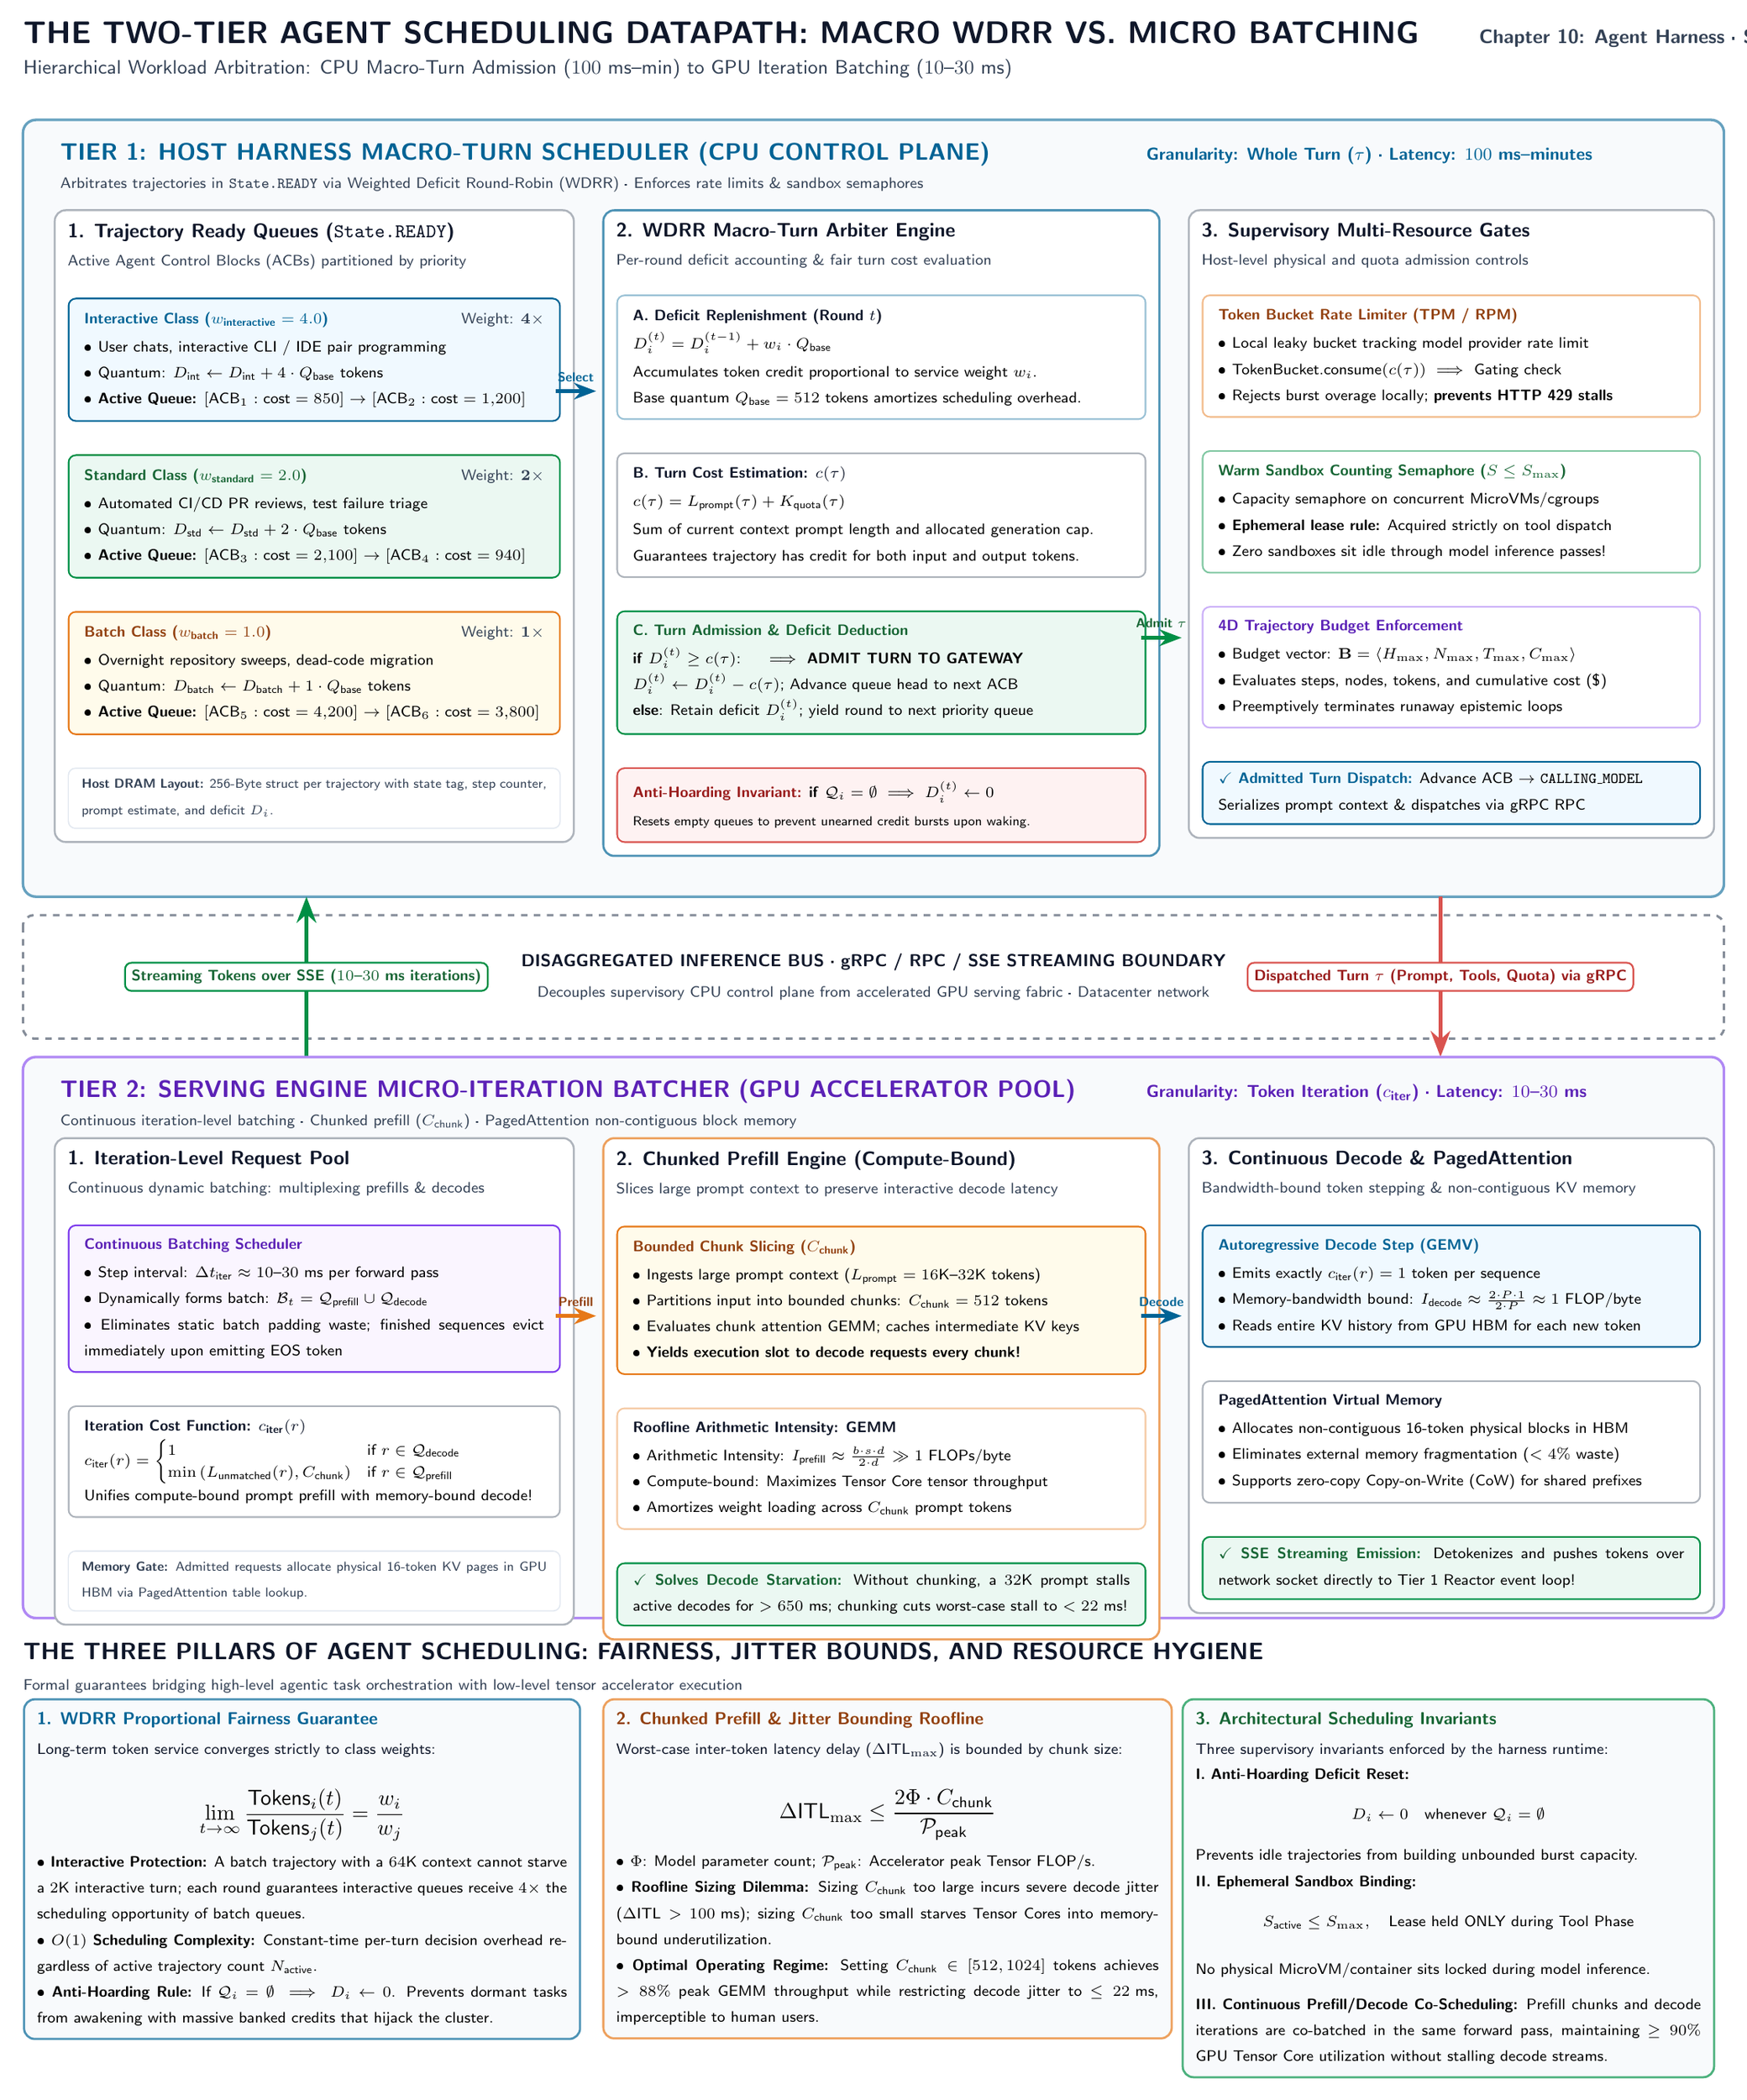
\begin{tikzpicture}[
  font=\sffamily,
  scale=1.0,
  >=Stealth,
  node distance=0.5cm
]

% -------------------------------------------------------------
% MASTER TITLE BANNER
% -------------------------------------------------------------
\node[anchor=north west, inner sep=0pt] (title) at (0, 33.2) {
  \begin{minipage}{27.6cm}
    \begin{tabular}{@{}p{23.2cm} r@{}}
      {\fontsize{13.5}{17}\selectfont \textbf{\textcolor{DarkSlate}{THE TWO-TIER AGENT SCHEDULING DATAPATH: MACRO WDRR VS. MICRO BATCHING}}} &
      \fontsize{9.5}{12}\selectfont \textcolor{slatesteel}{\textbf{Chapter 10: Agent Harness · Section 10.5}} \\[2pt]
      {\fontsize{9}{11.5}\selectfont \textcolor{slatesteel}{Hierarchical Workload Arbitration: CPU Macro-Turn Admission ($100\text{ ms}\text{--}\text{min}$) to GPU Iteration Batching ($10\text{--}30\text{ ms}$)}} & \\
    \end{tabular}
  \end{minipage}
};

% -------------------------------------------------------------
% TIER 1: HOST CPU MACRO-TURN SCHEDULER
% -------------------------------------------------------------
% Outer Container Box
\draw[draw=BlueLine!60, fill=coolparchment, line width=1.2pt, rounded corners=6pt] 
  (0, 31.6) rectangle (27.6, 19.0);

% Header inside Tier 1
\node[anchor=north west, inner sep=0pt] at (0.6, 31.25) {
  \begin{minipage}{26.4cm}
    \begin{tabular}{@{}p{17.2cm} r@{}}
      {\fontsize{11}{13}\selectfont \textbf{\textcolor{BlueLine}{TIER 1: HOST HARNESS MACRO-TURN SCHEDULER (CPU CONTROL PLANE)}}} &
      \fontsize{8}{10}\selectfont \textcolor{BlueLine}{\textbf{Granularity: Whole Turn ($\tau$) · Latency: $100\text{ ms}\text{--}\text{minutes}$}} \\[1pt]
      {\fontsize{7.5}{9.5}\selectfont \textcolor{slatesteel}{Arbitrates trajectories in \texttt{State.READY} via Weighted Deficit Round-Robin (WDRR) · Enforces rate limits \& sandbox semaphores}} & \\
    \end{tabular}
  \end{minipage}
};

% --- Tier 1, Column 1: Priority Ready Queues ---
\node[anchor=north west, fill=white, draw=slatesteel!40, line width=0.9pt, rounded corners=5pt, inner sep=6pt] 
  (t1_col1) at (0.5, 30.15) {
  \begin{minipage}{8.0cm}
    {\fontsize{9}{11}\selectfont \textbf{\textcolor{DarkSlate}{1. Trajectory Ready Queues (\texttt{State.READY})}}}\\[1pt]
    {\fontsize{7}{9}\selectfont \textcolor{slatesteel}{Active Agent Control Blocks (ACBs) partitioned by priority}}

    \vspace{5pt}
    % Queue 1: Interactive
    \begin{tcolorbox}[colback=BlueL0, colframe=BlueLine, arc=3pt, boxrule=0.8pt, left=4pt, right=4pt, top=3pt, bottom=3pt]
      {\fontsize{7.5}{9.5}\selectfont \textbf{\textcolor{BlueLine}{Interactive Class ($w_{\text{interactive}} = 4.0$)}}\hfill \textcolor{slatesteel}{Weight: $\mathbf{4\times}$}}\\[1pt]
      {\fontsize{6.8}{8.5}\selectfont
      \textbullet\ User chats, interactive CLI / IDE pair programming\\
      \textbullet\ Quantum: $D_{\text{int}} \leftarrow D_{\text{int}} + 4 \cdot Q_{\text{base}}$ tokens\\
      \textbullet\ \textbf{Active Queue:} $[\text{ACB}_1: \text{cost}=850] \to [\text{ACB}_2: \text{cost}=1{,}200]$
      }
    \end{tcolorbox}

    \vspace{3pt}
    % Queue 2: Standard
    \begin{tcolorbox}[colback=GreenL0, colframe=GreenLine, arc=3pt, boxrule=0.8pt, left=4pt, right=4pt, top=3pt, bottom=3pt]
      {\fontsize{7.5}{9.5}\selectfont \textbf{\textcolor{forestsage}{Standard Class ($w_{\text{standard}} = 2.0$)}}\hfill \textcolor{slatesteel}{Weight: $\mathbf{2\times}$}}\\[1pt]
      {\fontsize{6.8}{8.5}\selectfont
      \textbullet\ Automated CI/CD PR reviews, test failure triage\\
      \textbullet\ Quantum: $D_{\text{std}} \leftarrow D_{\text{std}} + 2 \cdot Q_{\text{base}}$ tokens\\
      \textbullet\ \textbf{Active Queue:} $[\text{ACB}_3: \text{cost}=2{,}100] \to [\text{ACB}_4: \text{cost}=940]$
      }
    \end{tcolorbox}

    \vspace{3pt}
    % Queue 3: Batch
    \begin{tcolorbox}[colback=OrangeL0, colframe=OrangeLine, arc=3pt, boxrule=0.8pt, left=4pt, right=4pt, top=3pt, bottom=3pt]
      {\fontsize{7.5}{9.5}\selectfont \textbf{\textcolor{warmochre}{Batch Class ($w_{\text{batch}} = 1.0$)}}\hfill \textcolor{slatesteel}{Weight: $\mathbf{1\times}$}}\\[1pt]
      {\fontsize{6.8}{8.5}\selectfont
      \textbullet\ Overnight repository sweeps, dead-code migration\\
      \textbullet\ Quantum: $D_{\text{batch}} \leftarrow D_{\text{batch}} + 1 \cdot Q_{\text{base}}$ tokens\\
      \textbullet\ \textbf{Active Queue:} $[\text{ACB}_5: \text{cost}=4{,}200] \to [\text{ACB}_6: \text{cost}=3{,}800]$
      }
    \end{tcolorbox}

    \vspace{3pt}
    % ACB Note
    \begin{tcolorbox}[colback=white, colframe=GridGray, arc=3pt, boxrule=0.6pt, left=3pt, right=3pt, top=2pt, bottom=2pt]
      {\fontsize{6.5}{8}\selectfont \textcolor{slatesteel}{\textbf{Host DRAM Layout:} 256-Byte struct per trajectory with state tag, step counter, prompt estimate, and deficit $D_i$.}}
    \end{tcolorbox}
  \end{minipage}
};

% --- Tier 1, Column 2: WDRR Arbiter Engine ---
\node[anchor=north west, fill=white, draw=BlueLine!70, line width=1.0pt, rounded corners=5pt, inner sep=6pt] 
  (t1_col2) at (9.4, 30.15) {
  \begin{minipage}{8.6cm}
    {\fontsize{9}{11}\selectfont \textbf{\textcolor{DarkSlate}{2. WDRR Macro-Turn Arbiter Engine}}}\\[1pt]
    {\fontsize{7}{9}\selectfont \textcolor{slatesteel}{Per-round deficit accounting \& fair turn cost evaluation}}

    \vspace{4pt}
    % Box 1: Deficit Replenishment
    \begin{tcolorbox}[colback=white, colframe=BlueLine!40, arc=3pt, boxrule=0.8pt, left=4pt, right=4pt, top=3pt, bottom=3pt]
      {\fontsize{7.5}{9.5}\selectfont \textbf{\textcolor{DarkSlate}{A. Deficit Replenishment (Round $t$)}}}\\[1pt]
      {\fontsize{6.8}{8.5}\selectfont
      $D_i^{(t)} = D_i^{(t-1)} + w_i \cdot Q_{\text{base}}$\\[1pt]
      Accumulates token credit proportional to service weight $w_i$.\\
      Base quantum $Q_{\text{base}} = 512\text{ tokens}$ amortizes scheduling overhead.
      }
    \end{tcolorbox}

    \vspace{3pt}
    % Box 2: Turn Cost Estimation
    \begin{tcolorbox}[colback=white, colframe=slatesteel!40, arc=3pt, boxrule=0.8pt, left=4pt, right=4pt, top=3pt, bottom=3pt]
      {\fontsize{7.5}{9.5}\selectfont \textbf{\textcolor{DarkSlate}{B. Turn Cost Estimation: $c(\tau)$}}}\\[1pt]
      {\fontsize{6.8}{8.5}\selectfont
      $c(\tau) = L_{\text{prompt}}(\tau) + K_{\text{quota}}(\tau)$\\[1pt]
      Sum of current context prompt length and allocated generation cap.\\
      Guarantees trajectory has credit for both input and output tokens.
      }
    \end{tcolorbox}

    \vspace{3pt}
    % Box 3: Admission & Deduction
    \begin{tcolorbox}[colback=GreenL0, colframe=GreenLine, arc=3pt, boxrule=0.8pt, left=4pt, right=4pt, top=3pt, bottom=3pt]
      {\fontsize{7.5}{9.5}\selectfont \textbf{\textcolor{forestsage}{C. Turn Admission \& Deficit Deduction}}}\\[1pt]
      {\fontsize{6.8}{8.5}\selectfont
      \textbf{if} $D_i^{(t)} \ge c(\tau)$: \quad $\implies$ \textbf{ADMIT TURN TO GATEWAY}\\
      \quad $D_i^{(t)} \leftarrow $ \smash{$D_i^{(t)} - c(\tau)$}; Advance queue head to next ACB\\
      \textbf{else}: Retain deficit $D_i^{(t)}$; yield round to next priority queue
      }
    \end{tcolorbox}

    \vspace{3pt}
    % Box 4: Anti-Hoarding Invariant
    \begin{tcolorbox}[colback=RedL0, colframe=RedLine, arc=3pt, boxrule=0.8pt, left=4pt, right=4pt, top=3pt, bottom=3pt]
      {\fontsize{7}{9}\selectfont \textbf{\textcolor{deepburgundy}{Anti-Hoarding Invariant:}} \textbf{if} $\mathcal{Q}_i = \emptyset \implies D_i^{(t)} \leftarrow 0$\\[1pt]
      {\fontsize{6.5}{8}\selectfont Resets empty queues to prevent unearned credit bursts upon waking.}}
    \end{tcolorbox}
  \end{minipage}
};

% --- Tier 1, Column 3: Supervisory Admission Gates ---
\node[anchor=north west, fill=white, draw=slatesteel!40, line width=0.9pt, rounded corners=5pt, inner sep=6pt] 
  (t1_col3) at (18.9, 30.15) {
  \begin{minipage}{8.1cm}
    {\fontsize{9}{11}\selectfont \textbf{\textcolor{DarkSlate}{3. Supervisory Multi-Resource Gates}}}\\[1pt]
    {\fontsize{7}{9}\selectfont \textcolor{slatesteel}{Host-level physical and quota admission controls}}

    \vspace{4pt}
    % Gate 1: Token Bucket Rate Limiter
    \begin{tcolorbox}[colback=white, colframe=OrangeLine!50, arc=3pt, boxrule=0.8pt, left=4pt, right=4pt, top=3pt, bottom=3pt]
      {\fontsize{7.5}{9.5}\selectfont \textbf{\textcolor{warmochre}{Token Bucket Rate Limiter (TPM / RPM)}}}\\[1pt]
      {\fontsize{6.8}{8.5}\selectfont
      \textbullet\ Local leaky bucket tracking model provider rate limit\\
      \textbullet\ $\text{TokenBucket.consume}(c(\tau)) \implies$ Gating check\\
      \textbullet\ Rejects burst overage locally; \textbf{prevents HTTP 429 stalls}
      }
    \end{tcolorbox}

    \vspace{3pt}
    % Gate 2: Sandbox Counting Semaphore
    \begin{tcolorbox}[colback=white, colframe=GreenLine!50, arc=3pt, boxrule=0.8pt, left=4pt, right=4pt, top=3pt, bottom=3pt]
      {\fontsize{7.5}{9.5}\selectfont \textbf{\textcolor{forestsage}{Warm Sandbox Counting Semaphore ($S \le S_{\max}$)}}}\\[1pt]
      {\fontsize{6.8}{8.5}\selectfont
      \textbullet\ Capacity semaphore on concurrent MicroVMs/cgroups\\
      \textbullet\ \textbf{Ephemeral lease rule:} Acquired strictly on tool dispatch\\
      \textbullet\ Zero sandboxes sit idle through model inference passes!
      }
    \end{tcolorbox}

    \vspace{3pt}
    % Gate 3: 4D Budget Vectors
    \begin{tcolorbox}[colback=white, colframe=PurpleLine!40, arc=3pt, boxrule=0.8pt, left=4pt, right=4pt, top=3pt, bottom=3pt]
      {\fontsize{7.5}{9.5}\selectfont \textbf{\textcolor{deeproyal}{4D Trajectory Budget Enforcement}}}\\[1pt]
      {\fontsize{6.8}{8.5}\selectfont
      \textbullet\ Budget vector: $\mathbf{B} = \langle H_{\max}, N_{\max}, T_{\max}, C_{\max} \rangle$\\
      \textbullet\ Evaluates steps, nodes, tokens, and cumulative cost (\$)\\
      \textbullet\ Preemptively terminates runaway epistemic loops
      }
    \end{tcolorbox}

    \vspace{3pt}
    % Dispatch Badge
    \begin{tcolorbox}[colback=BlueL0, colframe=BlueLine, arc=3pt, boxrule=0.8pt, left=4pt, right=4pt, top=2pt, bottom=2pt]
      {\fontsize{7}{9}\selectfont \textbf{\textcolor{BlueLine}{\checkmark\ Admitted Turn Dispatch:}} Advance $\text{ACB} \to \texttt{CALLING\_MODEL}$\\
      Serializes prompt context \& dispatches via gRPC RPC}
    \end{tcolorbox}
  \end{minipage}
};

% Horizontal Flow Arrows inside Tier 1 (placed in clear vertical gaps)
\draw[->, BlueLine, line width=1.6pt] (8.65, 27.2) -- (9.3, 27.2);
\node[text=BlueLine, font=\fontsize{6}{7}\selectfont\bfseries, above=1pt] at (8.97, 27.2) {Select};

\draw[->, GreenLine, line width=1.6pt] (18.15, 23.2) -- (18.8, 23.2);
\node[text=forestsage, font=\fontsize{6}{7}\selectfont\bfseries, above=1pt] at (18.47, 23.2) {Admit $\tau$};

% -------------------------------------------------------------
% DISAGGREGATION INTERFACE / NETWORK RPC BUS
% -------------------------------------------------------------
\draw[draw=slatesteel!60, fill=white, line width=1.1pt, dashed, rounded corners=5pt] 
  (0, 18.7) rectangle (27.6, 16.7);

\node[anchor=center] at (13.8, 17.7) {
  \begin{minipage}{13.5cm}
    \centering
    {\fontsize{8.5}{10.5}\selectfont \textbf{\textcolor{DarkSlate}{DISAGGREGATED INFERENCE BUS · gRPC / RPC / SSE STREAMING BOUNDARY}}}\\[2pt]
    {\fontsize{7}{8.5}\selectfont \textcolor{slatesteel}{Decouples supervisory CPU control plane from accelerated GPU serving fabric · Datacenter network}}
  \end{minipage}
};

% Inter-tier arrows with contained overlay labels
\draw[->, RedLine, line width=2.0pt] (23.0, 19.0) -- (23.0, 16.4);
\node[anchor=center, fill=white, draw=RedLine, line width=0.8pt, rounded corners=3pt, inner sep=3pt] 
  at (23.0, 17.7) {\fontsize{6.8}{8.5}\selectfont\textbf{\textcolor{deepburgundy}{Dispatched Turn $\tau$ (Prompt, Tools, Quota) via gRPC}}};

\draw[<-, GreenLine, line width=2.0pt] (4.6, 19.0) -- (4.6, 16.4);
\node[anchor=center, fill=white, draw=GreenLine, line width=0.8pt, rounded corners=3pt, inner sep=3pt] 
  at (4.6, 17.7) {\fontsize{6.8}{8.5}\selectfont\textbf{\textcolor{forestsage}{Streaming Tokens over SSE ($10\text{--}30\text{ ms}$ iterations)}}};

% -------------------------------------------------------------
% TIER 2: ACCELERATOR SERVING ENGINE
% -------------------------------------------------------------
% Outer Container Box
\draw[draw=PurpleLine!60, fill=coolparchment, line width=1.2pt, rounded corners=6pt] 
  (0, 16.4) rectangle (27.6, 7.3);

% Header inside Tier 2
\node[anchor=north west, inner sep=0pt] at (0.6, 16.05) {
  \begin{minipage}{26.4cm}
    \begin{tabular}{@{}p{17.2cm} r@{}}
      {\fontsize{11}{13}\selectfont \textbf{\textcolor{deeproyal}{TIER 2: SERVING ENGINE MICRO-ITERATION BATCHER (GPU ACCELERATOR POOL)}}} &
      \fontsize{8}{10}\selectfont \textcolor{deeproyal}{\textbf{Granularity: Token Iteration ($c_{\text{iter}}$) · Latency: $10\text{--}30\text{ ms}$}} \\[1pt]
      {\fontsize{7.5}{9.5}\selectfont \textcolor{slatesteel}{Continuous iteration-level batching · Chunked prefill ($C_{\text{chunk}}$) · PagedAttention non-contiguous block memory}} & \\
    \end{tabular}
  \end{minipage}
};

% --- Tier 2, Column 1: Continuous Batching Iteration Pool ---
\node[anchor=north west, fill=white, draw=slatesteel!40, line width=0.9pt, rounded corners=5pt, inner sep=6pt] 
  (t2_col1) at (0.5, 15.1) {
  \begin{minipage}{8.0cm}
    {\fontsize{9}{11}\selectfont \textbf{\textcolor{DarkSlate}{1. Iteration-Level Request Pool}}}\\[1pt]
    {\fontsize{7}{9}\selectfont \textcolor{slatesteel}{Continuous dynamic batching: multiplexing prefills \& decodes}}

    \vspace{5pt}
    % Box: Orca/vLLM continuous scheduler
    \begin{tcolorbox}[colback=PurpleL0, colframe=PurpleLine, arc=3pt, boxrule=0.8pt, left=4pt, right=4pt, top=3pt, bottom=3pt]
      {\fontsize{7.5}{9.5}\selectfont \textbf{\textcolor{deeproyal}{Continuous Batching Scheduler}}}\\[1pt]
      {\fontsize{6.8}{8.5}\selectfont
      \textbullet\ Step interval: $\Delta t_{\text{iter}} \approx 10\text{--}30\text{ ms}$ per forward pass\\
      \textbullet\ Dynamically forms batch: $\mathcal{B}_t = \mathcal{Q}_{\text{prefill}} \cup \mathcal{Q}_{\text{decode}}$\\
      \textbullet\ Eliminates static batch padding waste; finished sequences evict immediately upon emitting EOS token
      }
    \end{tcolorbox}

    \vspace{3pt}
    % Box: Iteration Cost Function
    \begin{tcolorbox}[colback=white, colframe=slatesteel!40, arc=3pt, boxrule=0.8pt, left=4pt, right=4pt, top=3pt, bottom=3pt]
      {\fontsize{7.5}{9.5}\selectfont \textbf{\textcolor{DarkSlate}{Iteration Cost Function: $c_{\text{iter}}(r)$}}}\\[1pt]
      {\fontsize{6.8}{8.5}\selectfont
      $c_{\text{iter}}(r) = \begin{cases}
      1 & \text{if } r \in \mathcal{Q}_{\text{decode}} \\
      \min\left(L_{\text{unmatched}}(r), C_{\text{chunk}}\right) & \text{if } r \in \mathcal{Q}_{\text{prefill}}
      \end{cases}$\\[2pt]
      Unifies compute-bound prompt prefill with memory-bound decode!
      }
    \end{tcolorbox}

    \vspace{3pt}
    % Box: HBM Block Allocator
    \begin{tcolorbox}[colback=white, colframe=GridGray, arc=3pt, boxrule=0.6pt, left=3pt, right=3pt, top=2pt, bottom=2pt]
      {\fontsize{6.5}{8}\selectfont \textcolor{slatesteel}{\textbf{Memory Gate:} Admitted requests allocate physical 16-token KV pages in GPU HBM via PagedAttention table lookup.}}
    \end{tcolorbox}
  \end{minipage}
};

% --- Tier 2, Column 2: Chunked Prefill Engine ---
\node[anchor=north west, fill=white, draw=OrangeLine!70, line width=1.0pt, rounded corners=5pt, inner sep=6pt] 
  (t2_col2) at (9.4, 15.1) {
  \begin{minipage}{8.6cm}
    {\fontsize{9}{11}\selectfont \textbf{\textcolor{DarkSlate}{2. Chunked Prefill Engine (Compute-Bound)}}}\\[1pt]
    {\fontsize{7}{9}\selectfont \textcolor{slatesteel}{Slices large prompt context to preserve interactive decode latency}}

    \vspace{5pt}
    % Box 1: Chunk Slicing Mechanism
    \begin{tcolorbox}[colback=OrangeL0, colframe=OrangeLine, arc=3pt, boxrule=0.8pt, left=4pt, right=4pt, top=3pt, bottom=3pt]
      {\fontsize{7.5}{9.5}\selectfont \textbf{\textcolor{warmochre}{Bounded Chunk Slicing ($C_{\text{chunk}}$)}}}\\[1pt]
      {\fontsize{6.8}{8.5}\selectfont
      \textbullet\ Ingests large prompt context ($L_{\text{prompt}} = 16\text{K}\text{--}32\text{K}$ tokens)\\
      \textbullet\ Partitions input into bounded chunks: $C_{\text{chunk}} = 512\text{ tokens}$\\
      \textbullet\ Evaluates chunk attention GEMM; caches intermediate KV keys\\
      \textbullet\ \textbf{Yields execution slot to decode requests every chunk!}
      }
    \end{tcolorbox}

    \vspace{3pt}
    % Box 2: Roofline & GEMM Efficiency
    \begin{tcolorbox}[colback=white, colframe=OrangeLine!40, arc=3pt, boxrule=0.8pt, left=4pt, right=4pt, top=3pt, bottom=3pt]
      {\fontsize{7.5}{9.5}\selectfont \textbf{\textcolor{DarkSlate}{Roofline Arithmetic Intensity: GEMM}}}\\[1pt]
      {\fontsize{6.8}{8.5}\selectfont
      \textbullet\ Arithmetic Intensity: $I_{\text{prefill}} \approx \frac{b \cdot s \cdot d}{2 \cdot d} \gg 1\text{ FLOPs/byte}$\\
      \textbullet\ Compute-bound: Maximizes Tensor Core tensor throughput\\
      \textbullet\ Amortizes weight loading across $C_{\text{chunk}}$ prompt tokens
      }
    \end{tcolorbox}

    \vspace{3pt}
    % Box 3: Jitter Elimination
    \begin{tcolorbox}[colback=GreenL0, colframe=GreenLine, arc=3pt, boxrule=0.8pt, left=4pt, right=4pt, top=2pt, bottom=2pt]
      {\fontsize{7}{9}\selectfont \textbf{\textcolor{forestsage}{\checkmark\ Solves Decode Starvation:}} Without chunking, a $32\text{K}$ prompt stalls active decodes for $> 650\text{ ms}$; chunking cuts worst-case stall to $< 22\text{ ms}$!}
    \end{tcolorbox}
  \end{minipage}
};

% --- Tier 2, Column 3: Continuous Decode Batcher & PagedAttention ---
\node[anchor=north west, fill=white, draw=slatesteel!40, line width=0.9pt, rounded corners=5pt, inner sep=6pt] 
  (t2_col3) at (18.9, 15.1) {
  \begin{minipage}{8.1cm}
    {\fontsize{9}{11}\selectfont \textbf{\textcolor{DarkSlate}{3. Continuous Decode \& PagedAttention}}}\\[1pt]
    {\fontsize{7}{9}\selectfont \textcolor{slatesteel}{Bandwidth-bound token stepping \& non-contiguous KV memory}}

    \vspace{5pt}
    % Box 1: Autoregressive Decode Step
    \begin{tcolorbox}[colback=BlueL0, colframe=BlueLine, arc=3pt, boxrule=0.8pt, left=4pt, right=4pt, top=3pt, bottom=3pt]
      {\fontsize{7.5}{9.5}\selectfont \textbf{\textcolor{BlueLine}{Autoregressive Decode Step (GEMV)}}}\\[1pt]
      {\fontsize{6.8}{8.5}\selectfont
      \textbullet\ Emits exactly $c_{\text{iter}}(r) = 1\text{ token per sequence}$\\
      \textbullet\ Memory-bandwidth bound: $I_{\text{decode}} \approx \frac{2 \cdot P \cdot 1}{2 \cdot P} \approx 1\text{ FLOP/byte}$\\
      \textbullet\ Reads entire KV history from GPU HBM for each new token
      }
    \end{tcolorbox}

    \vspace{3pt}
    % Box 2: PagedAttention KV Allocation
    \begin{tcolorbox}[colback=white, colframe=slatesteel!40, arc=3pt, boxrule=0.8pt, left=4pt, right=4pt, top=3pt, bottom=3pt]
      {\fontsize{7.5}{9.5}\selectfont \textbf{\textcolor{DarkSlate}{PagedAttention Virtual Memory}}}\\[1pt]
      {\fontsize{6.8}{8.5}\selectfont
      \textbullet\ Allocates non-contiguous 16-token physical blocks in HBM\\
      \textbullet\ Eliminates external memory fragmentation ($< 4\%$ waste)\\
      \textbullet\ Supports zero-copy Copy-on-Write (CoW) for shared prefixes
      }
    \end{tcolorbox}

    \vspace{3pt}
    % Box 3: Streaming SSE Emitter
    \begin{tcolorbox}[colback=GreenL0, colframe=GreenLine, arc=3pt, boxrule=0.8pt, left=4pt, right=4pt, top=2pt, bottom=2pt]
      {\fontsize{7}{9}\selectfont \textbf{\textcolor{forestsage}{\checkmark\ SSE Streaming Emission:}} Detokenizes and pushes tokens over network socket directly to Tier 1 Reactor event loop!}
    \end{tcolorbox}
  \end{minipage}
};

% Horizontal Flow inside Tier 2 (placed in clear vertical gaps)
\draw[->, OrangeLine, line width=1.6pt] (8.65, 12.2) -- (9.3, 12.2);
\node[text=warmochre, font=\fontsize{6}{7}\selectfont\bfseries, above=1pt] at (8.97, 12.2) {Prefill};

\draw[->, BlueLine, line width=1.6pt] (18.15, 12.2) -- (18.8, 12.2);
\node[text=BlueLine, font=\fontsize{6}{7}\selectfont\bfseries, above=1pt] at (18.47, 12.2) {Decode};

% -------------------------------------------------------------
% TIER 3: MATHEMATICAL DIVIDENDS & ARCHITECTURAL INVARIANTS
% -------------------------------------------------------------
\node[anchor=north west, inner sep=0pt] at (0, 6.9) {
  \begin{minipage}{27.6cm}
    {\fontsize{10.5}{12.5}\selectfont \textbf{\textcolor{DarkSlate}{THE THREE PILLARS OF AGENT SCHEDULING: FAIRNESS, JITTER BOUNDS, AND RESOURCE HYGIENE}}}\\[2pt]
    {\fontsize{7.5}{9.5}\selectfont \textcolor{slatesteel}{Formal guarantees bridging high-level agentic task orchestration with low-level tensor accelerator execution}}
  \end{minipage}
};

% Three Bottom Cards Side by Side
% --- Bottom Card 1: WDRR Proportional Fairness ---
\node[anchor=north west, fill=coolparchment, draw=BlueLine!70, line width=1.0pt, rounded corners=5pt, inner sep=6pt] 
  (bcard1) at (0, 6.0) {
  \begin{minipage}{8.6cm}
    {\fontsize{8.5}{10.5}\selectfont \textbf{\textcolor{BlueLine}{1. WDRR Proportional Fairness Guarantee}}}\\[2pt]
    {\fontsize{7}{9}\selectfont \textcolor{DarkSlate}{Long-term token service converges strictly to class weights:}}
    
    \vspace{3pt}
    \begin{equation*}
      \lim_{t \to \infty} \frac{\text{Tokens}_i(t)}{\text{Tokens}_j(t)} = \frac{w_i}{w_j}
    \end{equation*}
    
    {\fontsize{6.8}{8.5}\selectfont
    \textbullet\ \textbf{Interactive Protection:} A batch trajectory with a $64\text{K}$ context cannot starve a $2\text{K}$ interactive turn; each round guarantees interactive queues receive $4\times$ the scheduling opportunity of batch queues.\\
    \textbullet\ \textbf{$O(1)$ Scheduling Complexity:} Constant-time per-turn decision overhead regardless of active trajectory count $N_{\text{active}}$.\\
    \textbullet\ \textbf{Anti-Hoarding Rule:} If $\mathcal{Q}_i = \emptyset \implies D_i \leftarrow 0$. Prevents dormant tasks from awakening with massive banked credits that hijack the cluster.
    }
  \end{minipage}
};

% --- Bottom Card 2: Chunked Prefill Latency & Jitter ---
\node[anchor=north west, fill=coolparchment, draw=OrangeLine!70, line width=1.0pt, rounded corners=5pt, inner sep=6pt] 
  (bcard2) at (9.4, 6.0) {
  \begin{minipage}{8.8cm}
    {\fontsize{8.5}{10.5}\selectfont \textbf{\textcolor{warmochre}{2. Chunked Prefill \& Jitter Bounding Roofline}}}\\[2pt]
    {\fontsize{7}{9}\selectfont \textcolor{DarkSlate}{Worst-case inter-token latency delay ($\Delta \text{ITL}_{\max}$) is bounded by chunk size:}}
    
    \vspace{3pt}
    \begin{equation*}
      \Delta \text{ITL}_{\max} \le \frac{2 \Phi \cdot C_{\text{chunk}}}{\mathcal{P}_{\text{peak}}}
    \end{equation*}
    
    {\fontsize{6.8}{8.5}\selectfont
    \textbullet\ $\Phi$: Model parameter count; $\mathcal{P}_{\text{peak}}$: Accelerator peak Tensor FLOP/s.\\
    \textbullet\ \textbf{Roofline Sizing Dilemma:} Sizing $C_{\text{chunk}}$ too large incurs severe decode jitter ($\Delta \text{ITL} > 100\text{ ms}$); sizing $C_{\text{chunk}}$ too small starves Tensor Cores into memory-bound underutilization.\\
    \textbullet\ \textbf{Optimal Operating Regime:} Setting $C_{\text{chunk}} \in [512, 1024]$ tokens achieves $> 88\%$ peak GEMM throughput while restricting decode jitter to $\le 22\text{ ms}$, imperceptible to human users.
    }
  \end{minipage}
};

% --- Bottom Card 3: Three Invariants of Agent Scheduling ---
\node[anchor=north west, fill=coolparchment, draw=GreenLine!70, line width=1.0pt, rounded corners=5pt, inner sep=6pt] 
  (bcard3) at (18.8, 6.0) {
  \begin{minipage}{8.2cm}
    {\fontsize{8.5}{10.5}\selectfont \textbf{\textcolor{forestsage}{3. Architectural Scheduling Invariants}}}\\[2pt]
    {\fontsize{7}{9}\selectfont \textcolor{DarkSlate}{Three supervisory invariants enforced by the harness runtime:}}
    
    \vspace{3pt}
    {\fontsize{6.8}{8.5}\selectfont
    \textbf{I. Anti-Hoarding Deficit Reset:}
    \begin{equation*}
      D_i \leftarrow 0 \quad \text{whenever } \mathcal{Q}_i = \emptyset
    \end{equation*}
    Prevents idle trajectories from building unbounded burst capacity.\\[4pt]
    \textbf{II. Ephemeral Sandbox Binding:}
    \begin{equation*}
      S_{\text{active}} \le S_{\max}, \quad \text{Lease held ONLY during Tool Phase}
    \end{equation*}
    No physical MicroVM/container sits locked during model inference.\\[4pt]
    \textbf{III. Continuous Prefill/Decode Co-Scheduling:}
    Prefill chunks and decode iterations are co-batched in the same forward pass, maintaining $\ge 90\%$ GPU Tensor Core utilization without stalling decode streams.
    }
  \end{minipage}
};

\end{tikzpicture}
\end{document}
